\documentclass{beamer}
\mode<presentation>
{
\usepackage{dis-template}
}
\usepackage{listings}
\usepackage{hyperref}
\usepackage{textcomp}
\usepackage{soul}
\usepackage{color}
\definecolor{comments}{HTML}{50c878}
\lstset{language=C++,
  basicstyle=\ttfamily,
  keywordstyle=\color{blue}\ttfamily,
  stringstyle=\color{red}\ttfamily,
  commentstyle=\color{comments}\ttfamily,
  breaklines=true
}
\graphicspath{{slides/}} % TODO: eliminate this hack, necessary because scons builds at repository root

%---------------------------------------------------------------------
\titlepageinit{2}{Lab Equipment, Project Proposals}{28 \& 29 Jan 2015 (Week 2)}
%---------------------------------------------------------------------
\begin{document}
%---------------------------------------------------------------------
\begin{frame}
\titlepage

\setcounter{tocdepth}{1}
\tableofcontents
\end{frame}

% LAB PREPARATION
% Choose demo bench and ensure equipment and demos work
% Go through cars and prepare list of points to address

%---------------------------------------------------------------------
\section{Lab Equipment} % [10 mins]
%---------------------------------------------------------------------
\begin{frame}
\centering \huge Lab Equipment
\end{frame}

%---------------------------------------------------------------------
\subsection{Lab Power Supply}

\begin{frame}
\frametitle{Benchtop Power Supply Intro}
\begin{columns}[t]
\column{0.646\textwidth}
\begin{itemize}
  \item Provides a regulated power source
  \item Limits to the more restrictive of the voltage setpoint or current setpoint
  \item Or, a more helpful way to think about it:
  \begin{itemize}
    \item Acts as a constant voltage supply
    \item Until it hit the current setpoint (or ``current limit''), then it regulates the voltage not to exceed the current limit
    \item Set current limit to a known ``shouldn't exceed'' point to act as a fuse
  \end{itemize}
  \item Caveat: source has internal capacitance and limiting has response time
  \begin{itemize}
    \item May instantaneously exceed current limit
  \end{itemize}
\end{itemize}

\column{0.323\textwidth}
\begin{figure}
  \centering
  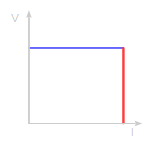
\includegraphics[width=1.0\columnwidth]{images-dis2/psu-iv} \newline
  IV Curve \\
  {\tiny \textcolor{blue}{constant-voltage mode}} \\
  {\tiny \textcolor{red}{current-limiting mode}}
\end{figure}
\end{columns}
\end{frame}

\begin{frame}
\frametitle{Check your Understanding}
\centering
So I've got a power supply set at $V_{set}$=5v, $I_{set}$=500mA \\
and some $\tfrac{1}{4}$-watt resistors... \\
\hfill \\
What will be the voltage across, current through, and \\
power supply operating regime when loaded with: \\
\hfill \\
100 $\Omega$ resistor \\ % 5v, 50mA, CV
\hfill \\
1 $\Omega$ resistor \\ % 0.5v, 500mA, CC / current limiting
\hfill \\
10 $\Omega$ resistor \\ % 5v, 500mA, CC/CV (either is fine), but vastly exceeds thermal limits (2.5w) and should start smelling funny
\pause
\scriptsize{why might this be a bad idea?}
% TODO: add resistor color code pictures
\end{frame}

%---------------------------------------------------------------------
\subsection{Function Generator}
\begin{frame}
\frametitle{Function Generator Intro}
\begin{columns}[t]
\column{0.646\textwidth}
\begin{itemize}
  \item Generates an arbitrary waveform with configurable parameters
  \item Useful for generating test inputs
  \begin{itemize}
    \item ... like motor driver PWM inputs
    \item ... and servo control signal
  \end{itemize}
  \item ``but wait, why not use my MCU?!''
  \begin{itemize}
    \item<2-> Debugging protip: test things in isolation!
    \item<2-> Function generator output is known good
    \item<2-> You are much less sure your software works the first time, every time
  \end{itemize}
\end{itemize}

\column{0.323\textwidth}
\begin{figure}
  \centering
  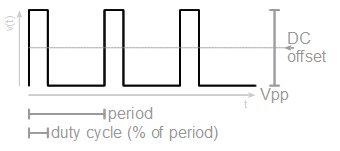
\includegraphics[width=1.0\columnwidth]{images-dis2/funcwave-square} \newline
  Square Wave
\end{figure}

\begin{figure}
  \centering
  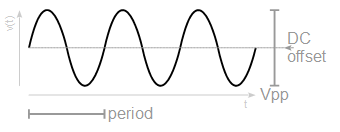
\includegraphics[width=1.0\columnwidth]{images-dis2/funcwave-sine} \newline
  Sine Wave
\end{figure}
% TODO: add triangle and sawtooth waves
\end{columns}
\end{frame}

\begin{frame}
\frametitle{50-ohm mode}
\begin{columns}[t]
\column{0.646\textwidth}
\begin{itemize}
  \item Function generators internally have a \\
  50$\Omega$ impedance and expect a 50$\Omega$ load
  \item Double the voltage is generated internally
  \begin{itemize}
    \item If you have a high impedance (Hi-Z) load, you see double the voltage
  \end{itemize}
  \item You can either:
  \begin{itemize}
    \item Manually halve the voltage \\
     - or -
    \item Set the generator into Hi-Z mode
  \end{itemize}
\end{itemize}

\column{0.323\textwidth}
\centering
\begin{figure}
  \centering
  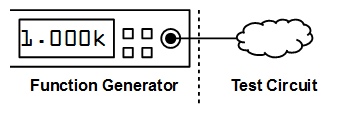
\includegraphics[width=0.75\columnwidth]{images-dis2/funcgen-header} \newline
  Function generator \\
  at setpoint $V_{set}$ \\
  \hfill \\
  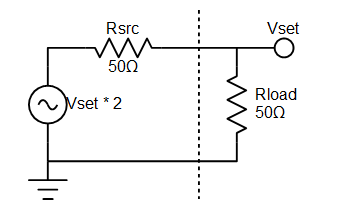
\includegraphics[width=0.75\columnwidth]{images-dis2/funcgen-50ohm} \newline
  with a 50$\Omega$ load
  
  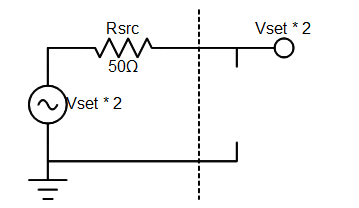
\includegraphics[width=0.75\columnwidth]{images-dis2/funcgen-hiz} \newline
  with a Hi-Z load
\end{figure}
\end{columns}
\end{frame}

%---------------------------------------------------------------------
\subsection{Oscilloscope}

\begin{frame}
\frametitle{Oscilloscope Intro}
\begin{columns}[t]
\column{0.646\textwidth}
\begin{itemize}
  \item Displays graph of voltage over time
  \begin{itemize}
    \item Well, no - - - -, Sherlock
  \end{itemize}
  \item<2-> Provides visibility into your system
  \item<2-> Verify signals are what you expect:
  \begin{itemize}
    \item Is your motor turning on?
    \item Is your speed sensor outputting counts?
  \end{itemize}
  \item<2-> Provide insights into subsystems:
  \begin{itemize}
    \item See how line camera output works
  \end{itemize}
  \item<2-> If you ever get stuck...
  \begin{itemize}
    \item Don't debug by brute force
    \item Turn on the scope and figure out the root of the problem
  \end{itemize}
\end{itemize}

\column{0.323\textwidth}
\begin{figure}
  \centering
  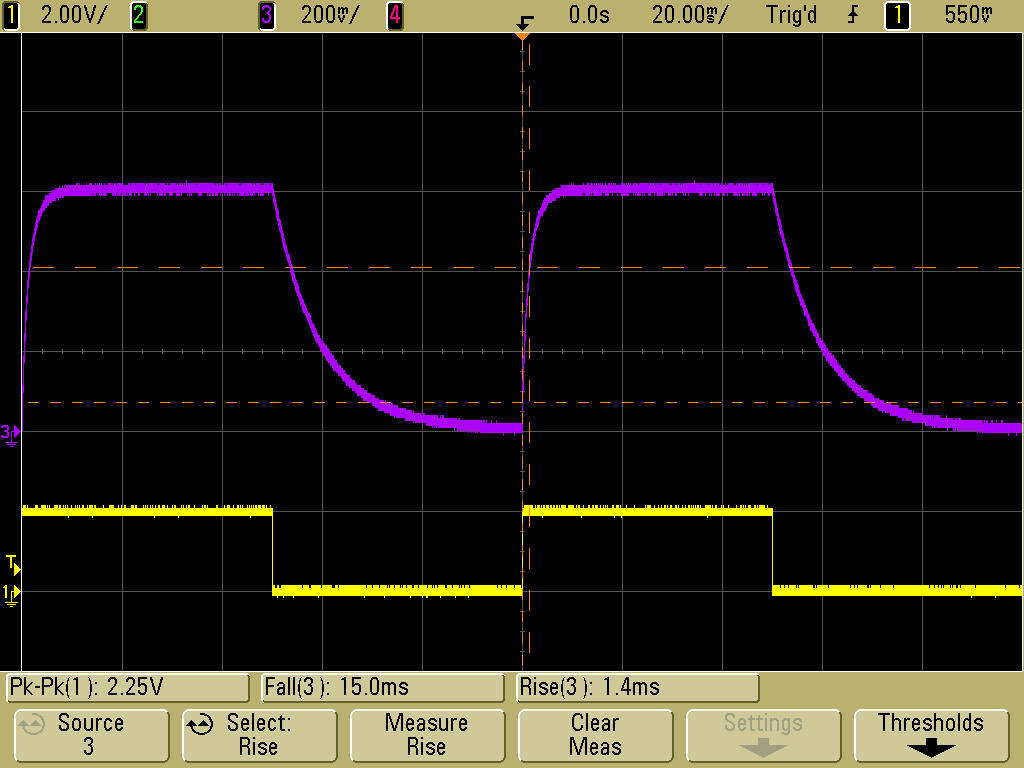
\includegraphics[width=1.0\columnwidth]{images-dis2/scope} \newline
  Scope traces
\end{figure}
\end{columns}
\end{frame}

\begin{frame}
\frametitle{Viewing Window}
\begin{columns}[t]
\column{0.646\textwidth}
\begin{itemize}
  \item There is an auto-scale function
  \begin{itemize}
    \item but garbage-in, garbage-out...
    \item and Prof. Pister will die a little inside...
  \end{itemize}
  \item Know how to manually set the scope
  \begin{itemize}
    \item You should have an idea of what to expect \\
    {\scriptsize you DO understand your circuit, right? RIGHT?!}
    \item Set the per-channel vertical scale based on the expected voltage range
    \item Set the global horizontal scale based on expected timescale
  \end{itemize}
  \item Capture modes
  \begin{itemize}
    \item Trigger: aligns start time to a signal edge
    \item Auto: continuous sampling
  \end{itemize}
\end{itemize}

\column{0.323\textwidth}
\begin{figure}
  \centering
  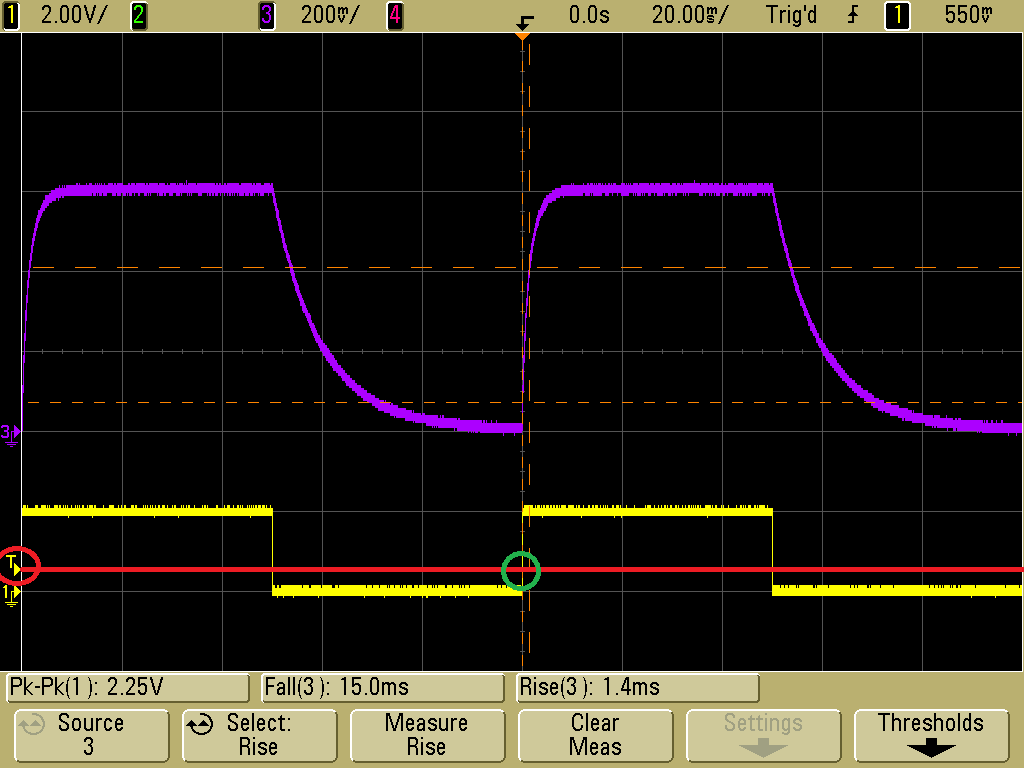
\includegraphics[width=1.0\columnwidth]{images-dis2/scope-trigger} \newline
  Triggering mode \\
  {\tiny trigger level setpoint in red} \\
  {\tiny triggered rising edge in green}
\end{figure}
\end{columns}
\end{frame}

\begin{frame}
\frametitle{Probe Compensation}
\begin{columns}[t]
\column{0.646\textwidth}
\begin{itemize}
  \item Scope has an internal input resistance \\
  and capacitance
  \item A 10:1 probe presents a higher input resistance by attenuation
  \begin{itemize}
    \item Most scopes can compensate for this
    \item Internally, a 9M$\Omega$ resistor forming a resistive divider with scope input
  \end{itemize}
  \item But need capacitive divider for AC signals
  \begin{itemize}
    \item Input capacitance varies with each scope
    \item Tunable capacitor on probe
  \end{itemize}
  \item Compensation procedure
  \begin{itemize}
    \item Connect probe to reference square wave
    \item Tune probe until wave is square
  \end{itemize}
\end{itemize}

\column{0.323\textwidth}
\begin{figure}
  \centering
  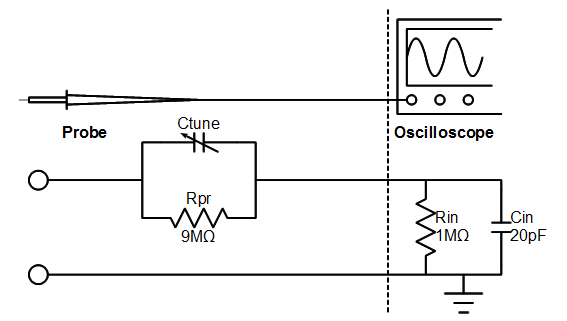
\includegraphics[width=1.0\columnwidth]{images-dis2/probe-internals} \newline
  Probe schematic \\
  {\scriptsize note divider circuit and tunable capacitor}
\end{figure}
\end{columns}
\hfill \\
\centering {\tiny Adapted from \url{http://www.syscompdesign.com/assets/Images/AppNotes/probes.pdf}}
% Additional reference with section on HF comp: https://www.picotech.com/library/application-note/how-to-tune-x10-oscilloscope-probes
\end{frame}

\begin{frame}
\frametitle{Check your Understanding}
\centering
Show me you know what you're doing! \\
\hfill \\
Generate a square wave with these characteristics \\
and show it on your scope: \\
\hfill \\
low voltage = 0v \\
high voltage = 5v \\
period = 10ms \\
high time = 2ms \\
\hfill \\
\begin{figure}
  \centering
  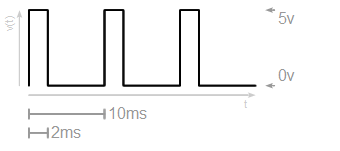
\includegraphics[width=0.4\columnwidth]{images-dis2/funcwave-square-task}
\end{figure}
\end{frame}

\begin{frame}
\frametitle{Questions?}
\centering
{\huge solid?} \\
\vspace{20px}
\tiny{we're all testing pros now, right?}
\end{frame}

%---------------------------------------------------------------------
\section{Project Proposals} % [5 mins]
%---------------------------------------------------------------------
\begin{frame}
\centering \huge Project Proposals
\end{frame}

\subsection{Overall Philosophy}

\begin{frame}
\frametitle{Focus: Planning \& Reliability}
\begin{columns}[t]
\column{0.646\textwidth}
\begin{itemize}
  \item \st{Measure once, cut twice, then hammer}
  \item Measure twice, cut once
  \item Start thinking about high-level project plan
  \begin{itemize}
    \item Plan ahead and examine feasibility
    \item Get feedback on design ideas
  \end{itemize}
  \item Reliability first, THEN performance
  \begin{itemize}
    \item ``Better is the enemy of the good''
    \item Fast car going into a wall gets you a \\ \href{http://tvtropes.org/pmwiki/pmwiki.php/Main/FMinusMinus}{F minus minus}
  \end{itemize}
\end{itemize}

\column{0.323\textwidth}
\begin{figure}
  \centering
  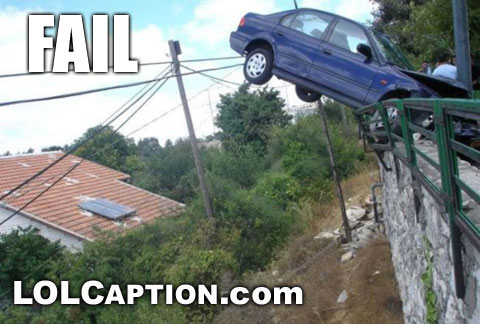
\includegraphics[width=1.0\columnwidth]{images-dis2/car-crash} \newline
  One weird trick \\
  to flunk ee192! \\
  {\tiny image from LOLCaption.com}
\end{figure}
\end{columns}
\end{frame}

%---------------------------------------------------------------------
\subsection{Mechanical Design}

\begin{frame}
\frametitle{Mechanical: Tips n' Tricks}
\begin{columns}[t]
\column{0.646\textwidth}
\begin{itemize}
  \item Goal: show us that you have a solid plan for mounting boards / other mechanisms
  \begin{itemize}
    \item Level of detail: screw holes, dimensions
  \end{itemize}
  \item Paper and pencil is acceptable
  \begin{itemize}
    \item Possibly even the most expedient solution
  \end{itemize}
  \item Cameraphone to take and annotate photos
  \item Draw over picture in Paint or PowerPoint
  \begin{itemize}
    \item Can even be physically accurate
  \end{itemize}
  \item SolidWorks only if you know how
  \begin{itemize}
    \item Parametric CAD is really, really nice, but not worth learning for this
  \end{itemize}
\end{itemize}

\column{0.323\textwidth}
\begin{figure}
  \centering
  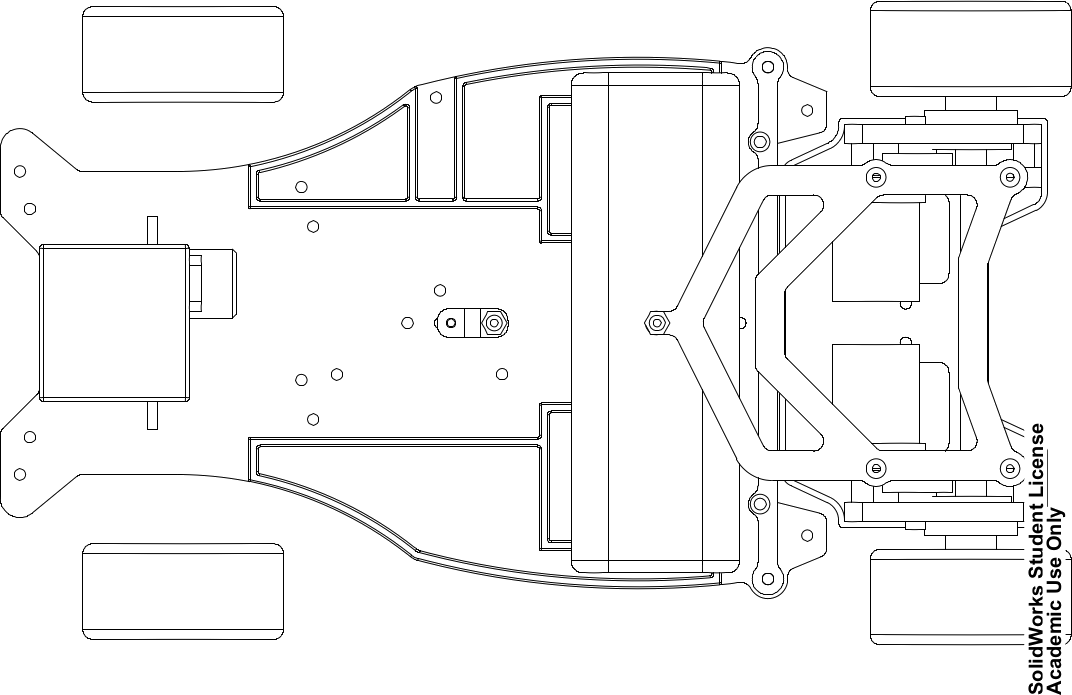
\includegraphics[width=1.0\columnwidth]{images-dis2/car-raster-top} \\
  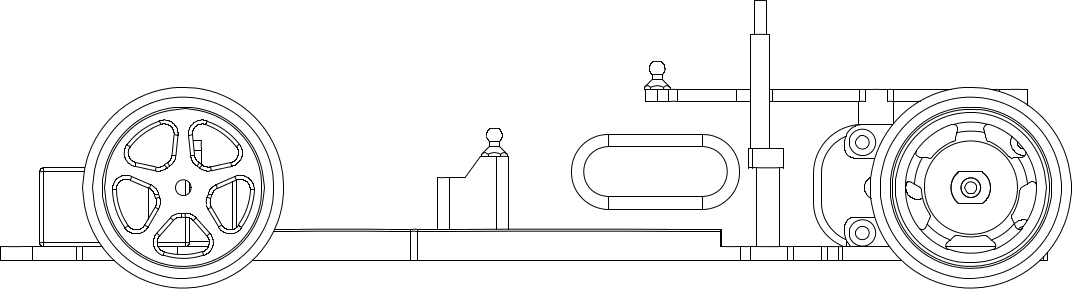
\includegraphics[width=1.0\columnwidth]{images-dis2/car-raster-side} \\
  Use the provided diagrams! \\
  Links:
  {\tiny
  \href{http://www-inst.eecs.berkeley.edu/~ee192/sp15/files/chassis-sketch-top-view.pdf}{(top)}
  \href{http://www-inst.eecs.berkeley.edu/~ee192/sp15/files/chassis-sketch-side-view.pdf}{(side)}
  \href{http://www-inst.eecs.berkeley.edu/~ee192/sp15/files/freescale_chassis_cad_sw.zip}{(CAD)}
  }
\end{figure}
\end{columns}
\end{frame}

%---------------------------------------------------------------------
\subsection{Electrical Design}

\begin{frame}
\frametitle{Electrical: Tips n' Tricks}
\begin{columns}[t]
\column{0.646\textwidth}
\begin{itemize}
  \item Goal: show us that you know motor driver design and have a board layout plan
  \begin{itemize}
    \item Please NO ROUTED BOARDS!
  \end{itemize}
  \item Quick demo: EAGLE schematic and layout
  \begin{itemize}
    \item Big idea: EDA tools are easy to use!
    \item Feel free to use better design software, like DipTrace or even KiCAD
  \end{itemize}
  \item And you can get them for free!
  \begin{itemize}
    \item ... as in beer: {\tiny
    \href{http://diptrace.com/}{(DipTrace)}
    \href{http://www.cadsoftusa.com/}{(EAGLE)}
    }
    \item ... as in speech: {\tiny
    \href{http://www.kicad-pcb.org/}{(KiCAD)}
    }
  \end{itemize}
  \item Tutorials for each can easily be found on the intertubes
\end{itemize}

\column{0.323\textwidth}
\begin{figure}
  \centering
  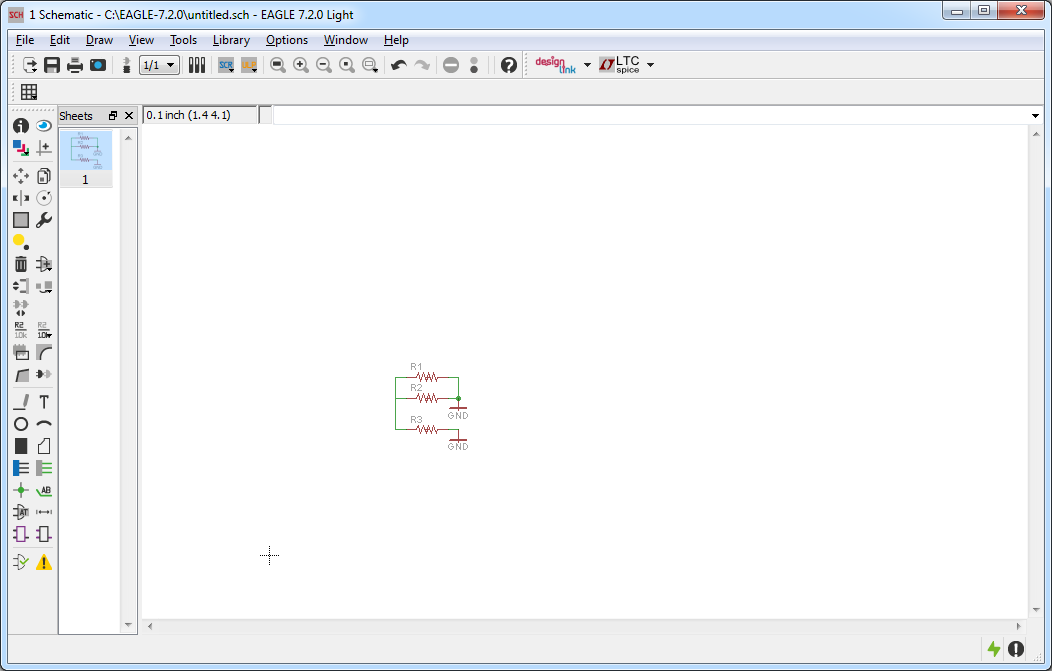
\includegraphics[width=0.8\columnwidth]{images-dis2/eagle-schematic} \\
  Schematic \\
  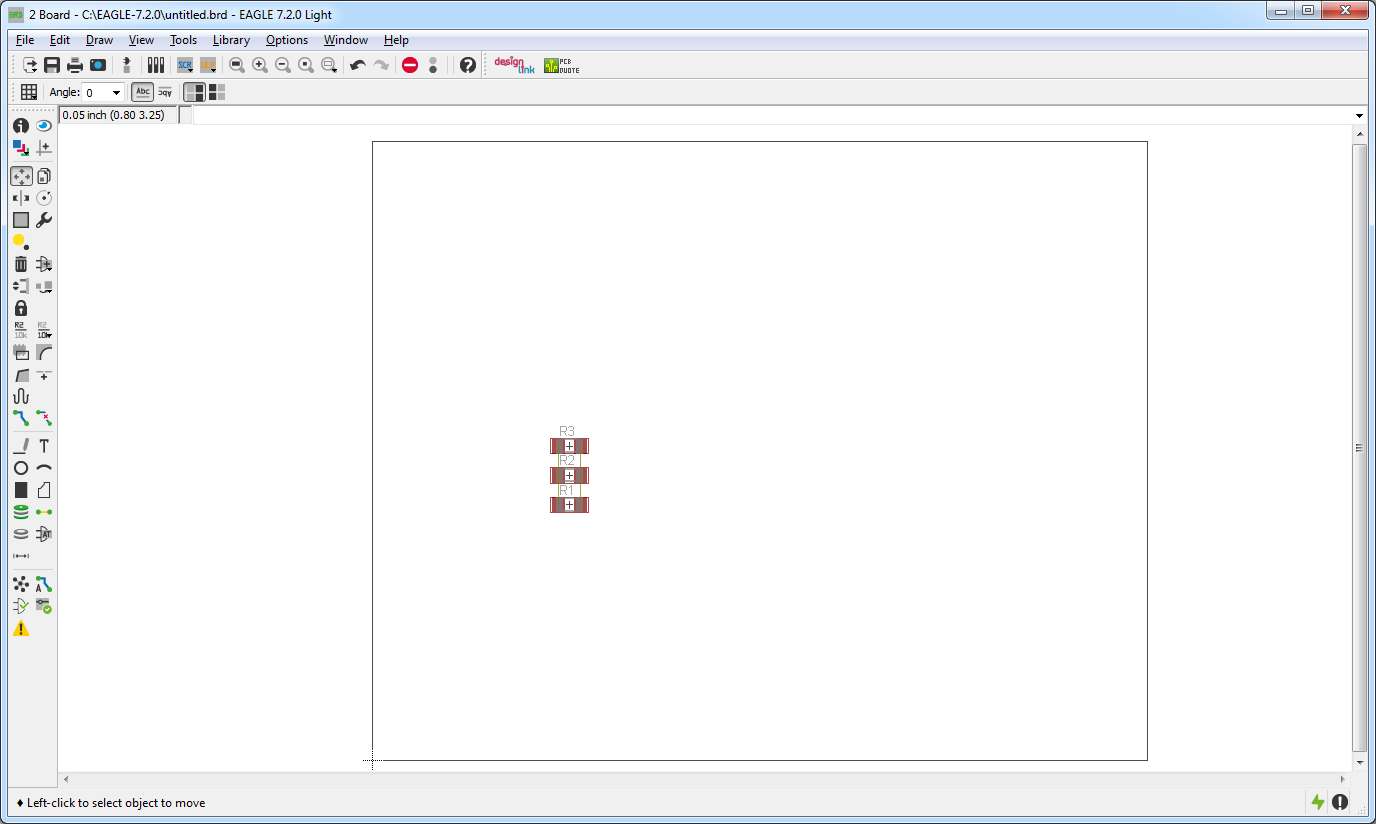
\includegraphics[width=0.8\columnwidth]{images-dis2/eagle-board} \\
  Board \\
  \hfill \\
  Library links: \
  {\tiny
  \href{http://www-inst.eecs.berkeley.edu/~ee192/sp15/files/ee192.lbr}{(lib 1)}
  \href{http://www-inst.eecs.berkeley.edu/~ee192/sp15/files/natcar.lbr}{(lib 2)}
  }
  {\tiny EAGLE only (for now!)}
\end{figure}
\end{columns}
\end{frame}

\begin{frame}
\frametitle{Schematic Style}
\begin{columns}[t]
\column{0.646\textwidth}
\begin{itemize}
  \item Style? Why do I care?!
  \begin{itemize}
    \item Confusing designs hide errors
    \item Helps reviewers understand your circuit
  \end{itemize}
  \item Component placement
  \begin{itemize}
    \item Dataflow ordering: left-to-right
    \item Voltages: high-to-low on top-to-bottom
  \end{itemize}
  \item Modularizing your schematic
  \begin{itemize}
    \item Use tunnels to minimize intersections \\ and decouple schematic blocks
    \item Use global voltage rails
  \end{itemize}
  \item Perfect is impossible
  \begin{itemize}
    \item ... but you CAN minimize stylistic badness
  \end{itemize}
\end{itemize}

\column{0.323\textwidth}
\begin{figure}
  \centering
  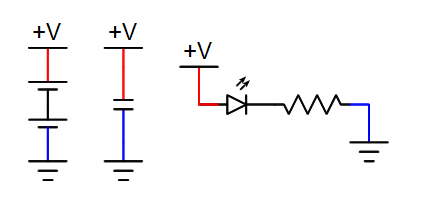
\includegraphics[width=1.0\columnwidth]{images-dis2/style-powerrails} \\
  Global power rails \\
  \hfill \\
  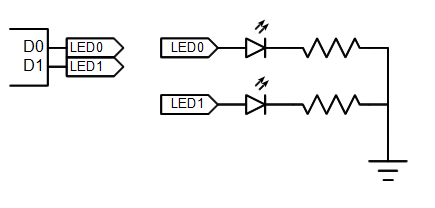
\includegraphics[width=1.0\columnwidth]{images-dis2/style-airwire} \\
  Decoupling using tunnels \\
\end{figure}
\end{columns}
\end{frame}

\begin{frame}
\frametitle{Questions?}
\centering
{\huge got it?} \\
\vspace{20px}
\tiny{we can all write awesome project proposals now, right?}
\end{frame}

%---------------------------------------------------------------------
\section{Car Critiques} % [5 mins prep + 10 mins discussion + 3x5 mins presentations = 35 mins]
%---------------------------------------------------------------------
\begin{frame}
\centering \huge Car Critiques
\end{frame}

\subsection{Theory}

\begin{frame}
\frametitle{Car Critiques}
\begin{columns}[t]
\column{0.646\textwidth}
\begin{itemize}
  \item Goal: don't reinvent the wheel
  \begin{itemize}
    \item Take design cues from those who came before you - recognize and use good ideas
    \item Conversely, learn from other's mistakes, \\ so you don't have to repeat them
  \end{itemize}
  \item Some design points to consider:
  \begin{itemize}
    \item Idiot-proofing
    \item Robustness
    \item Maintainability
    \item Design for Test
    \item Anything else you want to add?
  \end{itemize}
\end{itemize}

\column{0.323\textwidth}
\begin{figure}
  \centering
  
\includegraphics[width=1.0\columnwidth]{images-dis2/cereal-fire} \\
  It's been done before \\
  (don't repeat it!) \\
  {\tiny \textcopyright Fox}
\end{figure}
\end{columns}
\end{frame}

%---------------------------------------------------------------------
\subsection{Activity}

\begin{frame}
\frametitle{Group Car Critiques}
\centering
Break into your teams and critique your cars \\
{\tiny if your team doesn't have an assembled car, pair with one that does} \\
\hfill \\
Take 10 minutes to discuss amongst yourselves \\
{\tiny (I'll walk around to help out and offer suggestions!)} \\
then you'll present your findings to the class \\
{\tiny (aim for about 3 minutes, then we'll give others a chance to chime in)} \\
\hfill \\
\underline{Stuck? Consider these desirable features:} \\
{\footnotesize
\begin{columns}[t]
\column{0.45\textwidth}
  \centering
  Idiot-proofing \\
  {\tiny we're not idiots, but not everyone has had their coffee} \\
  Robustness \\
  {\tiny because, well, crash happens...}

\column{0.45\textwidth}
  \centering
  Maintainability \\
  {\tiny how can you make fixing a blown board easy?} \\
  Design for Test \\
  {\tiny things WILL go wrong; how do you make debug easy?} \\
\end{columns}
... and anything else you can think of ... \\
}
\end{frame}

\begin{frame}
\frametitle{Car Critique Presentations}
\centering
Start by introducing yourselves \\
{\tiny both as a team and as individuals} \\
\hfill \\
\underline{Then, talk about your car:} \\
What did you like about your car? Why? \\
What did not not like about your car? Why? \\
Did you see any good design philosophies? \\
Is there anything you would have done differently? \\
\end{frame}

%---------------------------------------------------------------------
\section{Soldering Refresher} % [5 mins]
%---------------------------------------------------------------------
% TODO: Perhaps next year.

% Quick interactive quiz:
% Everyone should be a pro now, right? Qualified on 0201?
% Diagram: soldering iron, component lead, reel, question marks

% Main goal of soldering: reliable electrical connection

% Need solder to flow onto and adhere to both component lead and board pad
% What might cause solder not to adhrere? How do we address it?

% Question: what affects thermal transfer? how do we address it?
% Cross-section area: use broad side of tips
% Oxidation: regularly clean up, properly maintain tip and plating

% Pass out practice boards
% Next week will have SMT boards?
% Optionally: soldering critiques on Friday checkoff / office hours!

\end{document}
